\subsection{Instalación}
\subsubsection{Dependencias}
Este programa ha sido comprobado con el intérprete  ``\textsl{GNU CLISP 2.49}''
no se garantiza un correcto funcionamiento con cualquier otro intérprete o
versión. Para compilar también es necesario el programa ``\textsl{make}''.

\subsubsection{Compilación}
Para compilar el código LISP del programa ejecutar el comando \texttt{make
blokus}, para generar esta documentación \texttt{make doc}. Si ejecuta el
comando \texttt{make} o \texttt{make all} se compilará el programa y se generará
la esta documentación.

\subsubsection{Ejecución} En el directorio raíz del proyecto, ejecutar el script
\texttt{./run.sh}. Para conseguir un mejor rendimiento, el código se compila
automáticamente antes de lanzar el programa.

\clearpage
\subsection{Cómo jugar}
\subsubsection{Menú de inicio}
\begin{figure}[ht]
	\centering
	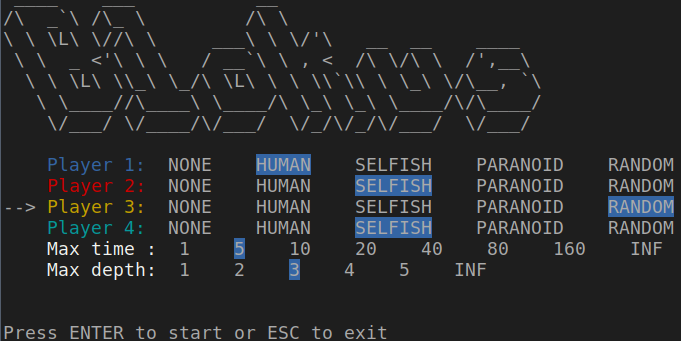
\includegraphics[width=\textwidth, keepaspectratio]{img/tui-init}
	\caption{Menú de inicio}
	\label{fig:menu_inicio}
\end{figure}

En esta pantalla (figura \ref{fig:menu_inicio}) se permite seleccionar el número
y tipo de jugadores, así como configurar los parámetros del algoritmo minimax.

Para navegar por el menu utilizar las flechas del teclado, para empezar la
partida pulsar la tecla RETURN y para salir la tecla ESC.

\subsubsection{Pantalla de juego}
\begin{figure}[ht]
	\centering
	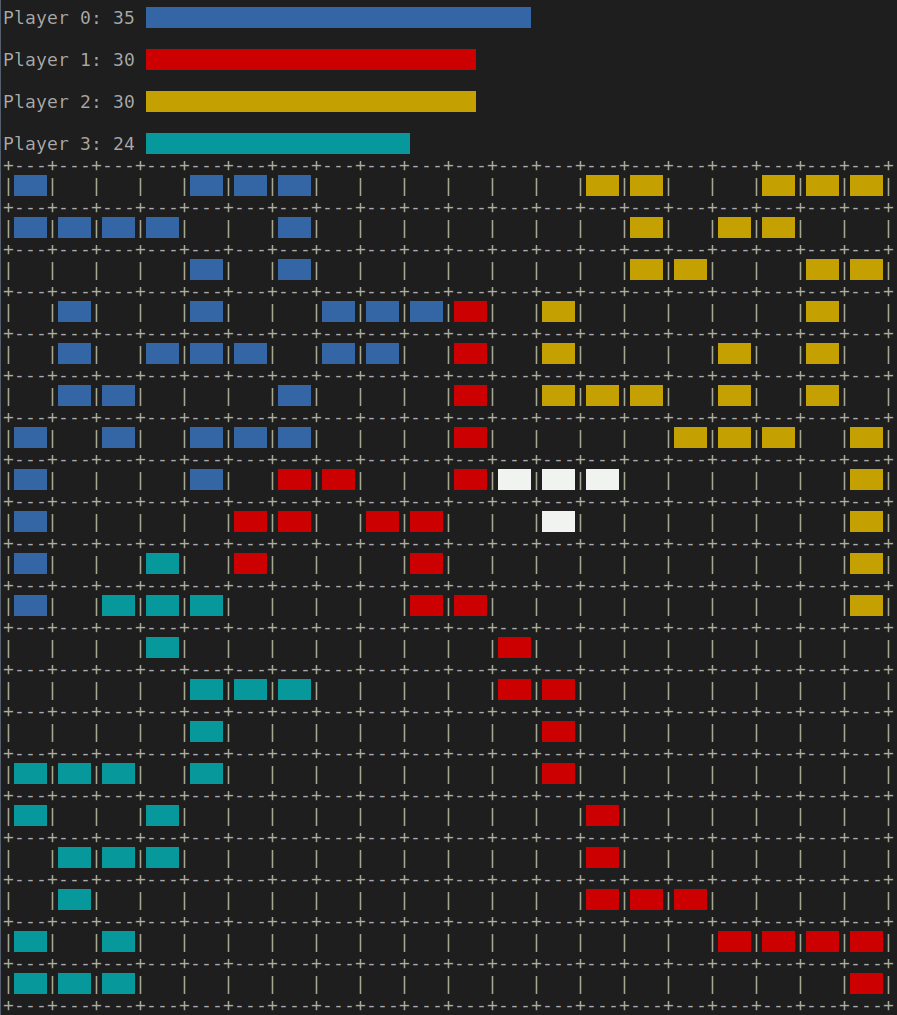
\includegraphics[width=\textwidth, height=0.6\textheight, keepaspectratio]{img/tui-game}
	\caption{Pantalla de juego}
	\label{fig:pantalla_juego}
\end{figure}

En la parte superior de esta pantalla (figura \ref{fig:pantalla_juego}) se puede
observar la puntación de cada jugador. El turno actual se indica mediante el
parpadeo del nombre del jugador.

En la parte inferior se muestra el tablero de juego. Las piezas de cada jugador
se representan con cuadrados rellenos de su respectivo color.

En el momento en el que llegue el turno de un jugador de tipo
``\textsl{humano}'' se le transfiere el control del teclado al usuario para que
pueda realizar su movimiento. La primera ficha disponible del jugador aparecerá
en la esquina superior izquierda, ésta será de color blanco hasta que se sitúe
en una posición válida, momento en el que se tornará al color del jugador. Las
teclas que permiten al usuario seleccionar, mover y posicionar sus fichas son
las siguientes:

\begin{itemize}
	\item \textbf{Flechas del teclado}: Movimiento de la pieza
	\item \textbf{R/r}: Rotar una pieza en sentido horario (r) o antihorario
		(R)
	\item \textbf{T/t}: Siguiente pieza (t) o anterior (T)
	\item \textbf{RETURN}: Colocar la pieza en la posición actual (solo se
		permitirá si la posición es válida)
	\item \textbf{ESC}: Cancelar la partida y volver al menú de inicio
\end{itemize}

Al final de la partida se muestra un texto parpadeante indicando el jugador
ganador.
